\chapter{Reinforcement learning}


\begin{description}
    \item[Reinforcement learning (RL)] \marginnote{Reinforcement learning (RL)}
        Learning a behavior (policy) by taking actions in a mutable environment that responds with rewards.

    \item[Policy] \marginnote{Policy}
        Probability distribution $\pi(a_t | s_t)$ that given the current state $s_t$ indicates 
        the likelihood of an action $a_t$.

    \item[Future cumulative reward] \marginnote{Future cumulative reward}
        Starting from a time step $t$, the future cumulative reward $R$ is the sum of all the local rewards $r_t$:
        \[ R = \sum_{i \geq 1} r_i \]

        \begin{description}
            \item[Future discounted cumulative reward] \marginnote{Future discounted cumulative reward} 
                Take into account the fact that future rewards are less certain than closer ones.
                \[ R = \sum_{i \geq 1} \gamma^{(i)} r_i \]
                where $0 <\gamma^{(i)} \leq 1$ is a discount factor that decreases exponentially over time.
        \end{description}

    \item[Markov decision process] \marginnote{Markov decision process}
        The environment can be modeled as a Markov decision process where future actions only depend on the current state.
        This is defined by the tuple $(\mathcal{S}, \mathcal{A}, \mathcal{R}, \mathcal{P}, \gamma)$
        where:
        \begin{itemize}
            \item $\mathcal{S}$ is the set of possible states.
            \item $\mathcal{A}$ is the set of possible actions.
            \item $\mathcal{R}$ is the set of rewards given state and action.
            \item $\mathcal{P}$ is the transition probability given state and action.
            \item $\gamma$ is the discount factor.
        \end{itemize}

    \item[RL problem] \marginnote{RL problem}
        Problem involving an agent that interacts with an environment.
        At each time step $t$, the following happens:
        \begin{enumerate}
            \item From the current state $s_t$, the agent selects an action $a_t$ according to a policy $\pi(a_t | s_t)$.
            \item The environment responds with a local reward $r_t \sim \mathcal{R}(r_t | s_t, a_t)$.
            \item The environment samples the next state $s_{t+1} \sim \mathcal{P}(s_{t+1} | s_t, a_t)$.
            \item The agent updates its policy accordingly.
        \end{enumerate}

        \begin{remark}
            A policy defines a trajectory:
            \[ (s_0, a_0) \mapsto (r_1, s_1, a_1) \mapsto \dots \]
        \end{remark}

    \item[Episode] \marginnote{Episode}
        Sequence of interactions between agent and environment from an initial state to a final state.

        \begin{remark}
            It is roughly the equivalent of an epoch.
        \end{remark}

    \item[Optimal policy] \marginnote{Optimal policy}
        Policy $\pi^*$ that maximizes the average future reward over all possible trajectories:
        \[ \pi^* = \arg\max_\pi \mathbb{E}\left[ \sum_{t \geq 0} \gamma^{(t)} r_t \right] \]

    \item[Model-based approach] \marginnote{Model-based}
        Method that needs to learn the transition probability $\mathcal{P}(s_{t+1} | s_t, a_t)$.

    \item[Model-free approach] \marginnote{Model-free}
        Method that only learns to make actions based on past experience.

        There are mainly two techniques:
        \begin{descriptionlist}
            \item[Value-based] \marginnote{Value-based}
                Learn a value function $V(s)$ that evaluates each state $s$.
                The policy is implicit, the best action is the one that brings to the state with the best evaluation.
            
            \item[Policy-based] \marginnote{Policy-based}
                Directly improve the probability distribution defined by the policy.
        \end{descriptionlist}
\end{description}



\section{$Q$-learning}

$Q$-learning is a value-based approach that learns a function $Q$ that acts as a proxy for the value function $V$.

\begin{description}
    \item[$Q$-value] \marginnote{$Q$-value}
        Measures the goodness of an action $a$ in the state $s$ by considering its future reward:
        \[ Q(s, a) = \mathbb{E}_{\substack{s_0 = s\\a_0 = a}} \left[ \sum_{t \geq 0} \gamma^{(t)} r_t \right] \]

    \item[Value function] \marginnote{Value function}
        Measures the goodness of a state $s$ by considering its future reward:
        \[ V(s) = \mathbb{E}_{s_0 = s} \left[ \sum_{t \geq 0} \gamma^{(t)} r_t \right] \]

        Given $Q$, $V$ can be computed as:
        \[ V(s) = \sum_{a} \pi(a | s) Q (s, a) \]

        \begin{remark}
            Given $V$, $Q$ can be computed as:
            \[ Q(s_t, a_t) = \sum_{s_{t+1}} \mathcal{P}(s_{t+1} | s_t, a_t) V(s_{t+1}) \]
            but this requires a model-based approach as $\mathcal{P}$ is needed.
        \end{remark}

    \item[Optimal $Q$-value] \marginnote{Optimal $Q$-value}
        The optimal $Q$-value $Q^*$ is the one that maximizes the expected cumulative reward 
        achievable starting from state $s$ with action $a$:
        \[ Q^*(s, a) = \max_\pi \mathbb{E}_{\substack{s_0 = s\\a_0 = a}} \left[ \sum_{t \geq 0} \gamma^{(t)} r_t \right] \]

    \item[Optimal policy] \marginnote{Optimal policy}
        The optimal policy $\pi^*$ is the one that makes the best action according to the optimal $Q$-value $Q^*$.
\end{description}


\subsection{Training}
\begin{description}
    \item[Bellman equation] \marginnote{Bellman equation}
        Expresses the optimal $Q$-value in terms of subproblems:
        \[ Q^*(s_t, a_t) = \mathbb{E}_{s_{t+1}} \left[ r_t + \gamma \max_{a_{t+1}} Q^*(s_{t+1}, a_{t+1}) \right] \]
        where $\max_{a_{t+1}} Q^*(s_{t+1}, a_{t+1}) = R_{s_{t+1}} = V^*(s_{t+1})$ is the optimal future cumulative reward from $s_{t+1}$ with action $a_{t+1}$.

        $Q^*$ can then be iteratively computed as follows:
        \[ Q^{(i+1)}(s_t, a_t) = Q^{(i)}(s_t, a_t) + \alpha\left( r_t + \gamma \max_{a_{t+1}} Q^{(i)}(s_{t+1}, a_{t+1}) - Q^{(i)}(s_t, a_t) \right) \]
        where:
        \begin{itemize}
            \item $\alpha$ is the learning rate.
            \item The update step aims to impose: 
                \[ Q^{(i)}(s_t, a_t) = r_t + \gamma \max_{a_{t+1}} Q^*(s_{t+1}, a_{t+1}) \]
                (i.e. respect the Bellman equation).
        \end{itemize}

    \item[$Q$-learning transition] \marginnote{$Q$-learning transition}
        Tuple of form:
        \[ (s_t, a_t, r_t, T, s_{t+1}) \]
        where:
        \begin{itemize}
            \item $s_t$ is the current state.
            \item $a_t$ is the action performed at the current step.
            \item $r_t$ is the reward at the current step.
            \item $T$ is a boolean indicating if the episode has ended.
            \item $s_{t+1}$ is the next state after performing the action $a_t$.
        \end{itemize}

        
        \item[Experience replay] \marginnote{Experience replay}
        For training, transitions are collected in a buffer by exploring the environment.
        Collected transitions can be replayed in any order, this has the advantage of:
        \begin{itemize}
            \item Avoid using correlated consecutive samples.
            \item Avoid biases caused by the exploitation of unbalanced transitions.
        \end{itemize}

        \begin{remark}
            $Q$-learning is an off-policy method. Training does not rely on a policy and only needs local transitions.
        \end{remark}

    \item[Epsilon greedy strategy] \marginnote{Epsilon greedy strategy}
        Introduce an exploration rate $\varepsilon$, initially set to 1 and progressively reduced during training.
        $\varepsilon$ is the probability of choosing a random action (exploration) instead of choosing the best-known action (exploitation).

    \item[Algorithm] \marginnote{$Q$-learning training}
        Given:
        \begin{itemize}
            \item A $Q$-table (to store the $Q$-values $Q(s, a)$), 
            \item A replay buffer $D$,
            \item The initial state $s_0$,
            \item The learning rate $\alpha$ and the discount factor $\gamma$,
            \item The exploration rate $\varepsilon$, 
        \end{itemize}
        an episode of $Q$-learning training does the following:
        \begin{itemize}
            \item Until the episode is not ended:
            \begin{enumerate}
                \item Choose the next action as:
                    \[ a_t = \begin{cases}
                        \texttt{random}(\mathcal{A}) & \text{with probability $\varepsilon$} \\
                        \max_a Q(s_t, a) & \text{with probability $1-\varepsilon$} \\
                    \end{cases} \]
                \item Perform $a_t$ and observe the reward $r_t$ and the next state $s_{t+1}$.
                \item Store $(s_t, a_t, r_t, T, s_{t+1})$ in $D$.
                \item Sample a random mini-batch $B$ from $D$. For each transition in $B$:
                \begin{enumerate}
                    \item Estimate the cumulative future reward:
                        \[ R = \begin{cases}
                            r_t & \text{if the episode is terminated} \\
                            r_t + \gamma \max_{a_{t+1}} Q(s_{t+1}, a_{t+1}) & \text{otherwise} \\
                        \end{cases} \]
                    \item Update the $Q$-table as:
                        \[ Q(s_t, a_t) = Q(s_t, a_t) + \alpha(R - Q(s_t, a_t)) \]
                \end{enumerate}
                \item Decrement $\varepsilon$.
            \end{enumerate}
        \end{itemize} 
\end{description}

\begin{remark}
    $Q$-learning requires to compute every possible state-action pair.
\end{remark}



\section{Deep $Q$-learning (DQN)}
\marginnote{Deep $Q$-learning (DQN)}

Use a neural network to estimate the optimal $Q$-value:
\[ Q(s, a, \matr{\theta}) \approx Q^*(s, a) \]

\begin{remark}
    In practice, the network outputs a value for each possible action.
\end{remark}

\begin{description}
    \item[Loss function] \marginnote{Loss function}
        The loss function for deep $Q$-learning is:
        \[ \mathcal{L}(\matr{\theta}) = \left( \mathbb{E}_{s'}[r_0 + \gamma \max_{a'} Q(s', a', \matr{\theta})] - Q(s, a, \matr{\theta}) \right)^2 \]
        where $\mathbb{E}_{s'}[r_0 + \gamma \max_{a'} Q(s', a', \matr{\theta})]$ is the expected value given by the Bellman equation and is an approximation of the target $Q^*$ (see more in \Cref{sec:dqn_improvements}).

        \begin{remark}
            As in traditional $Q$-learning, experience replay is used.
        \end{remark}
\end{description}

\begin{example}[Atari games]
    DQN successfully plays Atari games using an architecture composed of convolutions and feed-forward layers.
    The network takes as input the last $4$ frames of the game and outputs a $Q$-value for each of the possible actions. 

    \begin{figure}[H]
        \centering
        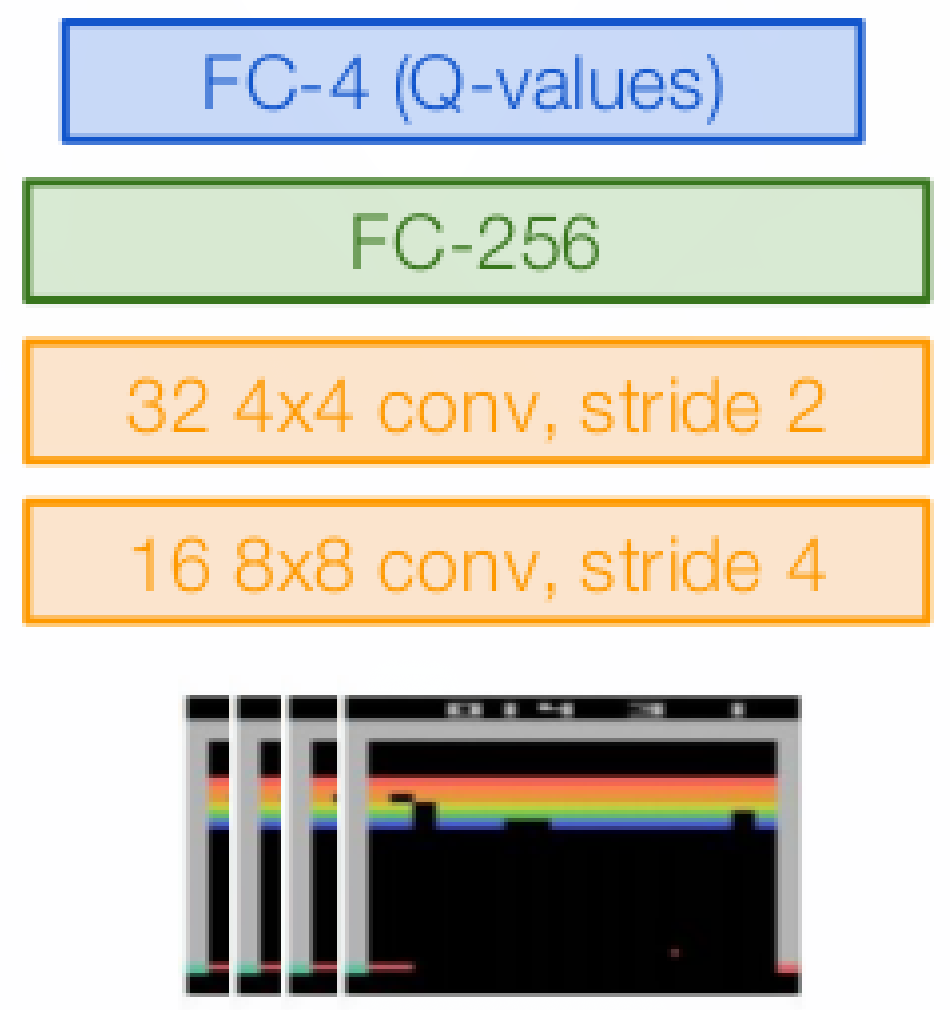
\includegraphics[width=0.2\linewidth]{./img/dqn_atari.png}
    \end{figure}

    A stack of images is necessary to capture movement. An LSTM layer can be used as an alternative.

    Instead of video screenshots, a dump of the RAM can be also used (e.g. the Atari 2600 console has 128 bytes of RAM).

    To adapt the reward for different games, a positive reward is encoded as $1$, a negative reward as $-1$ and a neutral reward as $0$. In other words, the amount of reward does not matter.
\end{example}


\subsection{Improvements} \label{sec:dqn_improvements}

\begin{description}
    \item[Fixed $Q$-targets] \marginnote{Fixed $Q$-targets}
        In the loss function, the same network computes the approximation of the target $Q^*$ ($\mathbb{E}_{s'}[r_0 + \gamma \max_{a'} Q(s', a', \matr{\theta})]$) and the current estimation ($Q(s, a, \matr{\theta})$).
        During training, both components change and this might lead to big oscillations.

        Fixed $Q$-targets uses a different network with parameters $\bar{\matr{\theta}}$ to compute the approximated target:
        \[ \mathbb{E}_{s'}[r_0 + \gamma \max_{a'} Q(s', a', \bar{\matr{\theta}})] - Q(s, a, \matr{\theta}) \]
        Periodically, the parameters $\matr{\theta}$ are copied in $\bar{\matr{\theta}}$.

    
    \item[Double $Q$-learning] \marginnote{Double $Q$-learning}
        The approximation of the target $Q^*$ is computed using the action that maximizes $Q$ and can therefore be an overestimation of the correct value.

        In double $Q$-learning, the choice of the action and its evaluation are decoupled into two networks $\matr{\theta}^\alpha$ and $\matr{\theta}^\beta$. At each training step, one of them is randomly chosen to select the action and the other estimates the target. For instance, if $\matr{\theta}^\alpha$ is chosen for selecting the action:
        \[
            \begin{split}
                a^* &= \max_a Q(s', a, \matr{\theta}^\alpha) \\
                Q(s, a, \matr{\theta}^\alpha) &= Q(s, a, \matr{\theta}^\alpha) + \alpha \left( r + Q(s, a^*, \matr{\theta}^\beta) - Q(s, a, \matr{\theta}^\alpha) \right) 
            \end{split}
        \]

    \item[Prioritized experience replay] \marginnote{Prioritized experience replay}
        Weight transitions with a large difference between predicted and expected target so that they are more likely to be sampled.
        Given a transition $t = (s, a, r, F, s')$, its update is given by:
        \[ \delta_t = r + \gamma \max_{a'} Q(s', a') - Q(s, a) \]
        
        The priority of $t$ can be defined as:
        \[ p_t = \vert \delta_t \vert \]
        and the probability of choosing $t$ is given by:
        \[ P_t = \frac{p_t^\alpha}{\sum_{t'} p_{t'}^\alpha} \]
        where $\alpha$ is a hyperparameter. If $\alpha=0$ all transitions have the same probability. If $\alpha$ is large, it privileges transitions with a high priority.

        \begin{description}
            \item[Importance sampling weights]
                By prioritizing a subset of transitions, there is the risk of overfitting them. Importance sampling weights can be used to fix the bias by changing the amount of update.

                Given a replay buffer of $N$ transitions, the weight for the transition $t$ is given by:
                \[ w_t = (N \cdot P_t)^{-\beta} \]
                where $\beta$ is initialized to $1$ and goes to $0$ during training. With $\beta \sim 1$, the weight compensates non-uniform sample probabilities.
                
                In practice, the weight is applied to the update value as:
                \[ \frac{w_t}{\max_{t'} w_{t'}} \delta_t \]
                where the denominator is a normalization factor.
        \end{description}


    \item[Dueling] \marginnote{Dueling}
        Decompose $Q(s, a)$ into two components:
        \begin{descriptionlist}
            \item[Value] $V(s)$ evaluates the state $s$.
            \item[Advantage] $A(s, a)$ evaluates the action $a$ in $s$ compared to all the other actions.
        \end{descriptionlist}

        Different strategies can be used to aggregate the two components:
        \begin{descriptionlist}
            \item[Naive aggregation]
                \[ Q(s, a) = V(s) + A(s, a) \]
                This approach does not allow to distinguish $V(s)$ and $A(s, a)$ from $Q(s, a)$. This makes it difficult to distribute the error during backpropagation.

            \item[Max aggregation]
                \[ Q(s, a) = V(s) + A(s, a) - \max_a A(s, a) \]
                This forces the advantage to be $0$ when the best action is selected.

            \item[Mean aggregation]
                \[ Q(s, a) = V(s) + A(s, a) - \underset{a}{\text{mean}}\, A(s, a) \]
                This has been empirically shown to be more stable.
        \end{descriptionlist}

    
    \item[Noisy networks] \marginnote{Noisy networks}
        Instead of traditional dense layers, use a noisy variation defined as:
        \[ y = \Big( \vec{b} + \matr{W}\vec{x} \Big) + \Big( (\vec{b}_\text{noisy} \odot \varepsilon^\vec{b}) + (\matr{W}_\text{noisy} \odot \varepsilon^\matr{W}) \vec{x} \Big) \]
        where:
        \begin{itemize}
            \item $\matr{W}$ and $\vec{b}$ are the parameters of a traditional dense layer.
            \item $\matr{W}_\text{noisy}$ and $\vec{b}_\text{noisy}$ are the parameters of the noisy stream.
            \item $\varepsilon^\vec{b}$ and $\varepsilon^\matr{W}$ are randomly generated noise.
        \end{itemize}

        The noise component adds randomicity in the choice of actions. Moreover, as noisy weights are learned, the network can learn to randomly explore the environment with different paces depending on the state.

        \begin{remark}
            Noisy networks empirically work better than the $\varepsilon$-greedy strategy.
        \end{remark}

    
    \item[Distributional RL] \marginnote{Distributional RL}
        Learn the probability distribution of the future cumulative reward instead of its expected value.
\end{description}



\section{Policy gradient techniques}

\begin{remark}
    $Q$-learning is a 1-step method that only updates the value of the state-action pair $(s, a)$ that led to the reward, ignoring all other state-action pairs that led to that state.
\end{remark}

\begin{description}
    \item[Off-policy techniques] \marginnote{Off-policy techniques}
        Methods that only use local transitions, without a policy (e.g. $Q$-learning).

    \item[On-policy techniques] \marginnote{On-policy techniques}
        Methods that try to improve the current policy.
\end{description}


\subsection{State-Action-Reward-State-Action (SARSA)}

\begin{description}
    \item[Update] \marginnote{State-Action-Reward-State-Action (SARSA)}
        An update for SARSA is defined as follows:
        \[ Q(s_t, a_t) = Q(s_t, a_t) + \alpha \left( r_t + Q(s_{t+1}, a_{t+1}) - Q(s_t, a_t) \right) \]
        differently from $Q$-learning that uses the best action ($\gamma\max_aQ(s_{t+1}, a)$) to estimate the target, in SARSA the actual action ($Q(s_{t+1}, a_{t+1})$) is used.

    \item[Transition]
        A transition in SARSA is defined as a mini-trajectory of two steps:
        \[ (s_i, a_i, r_i, s_{i+1}, a_{i+1}) \]
\end{description}


\subsection{Policy gradient methods}
\marginnote{Policy gradient methods}

Given a class of parametrized policies $\Pi = \{ \pi_\matr{\theta} \}$, a value for a policy $\pi_\matr{\theta}$ can be defined as:
\[ \mathcal{J}(\matr{\theta}) = \mathbb{E} \left[ \sum_{t \geq 0} \gamma^t r_t \right] \]

The optimal policy is the one such that:
\[ \matr{\theta}^* = \arg\max_\matr{\theta} \mathcal{J}(\matr{\theta}) \]

\begin{description}
    \item[REINFORCE] \marginnote{\textsc{Reinforce}}
        Given a sampled trajectory, \textsc{Reinforce} updates the parameters in the direction:
        \[ \Delta_\matr{\theta} = \nabla_\matr{\theta} \log \pi(a_t | s_t, \matr{\theta}) R_t \]

        \begin{description}
            \item[Baseline] \marginnote{Baseline}
                As the raw value of a trajectory is not meaningful, a baseline (i.e. expected reward) that depends on the state is added:
                \[ \Delta_\matr{\theta} = \nabla_\matr{\theta} \log \pi(a_t | s_t, \matr{\theta}) (R_t - b(s_t)) \]

                \begin{description}
                    \item[Actor-critic architecture] \marginnote{Actor-critic architecture}
                        The baseline is chosen as the value function:
                        \[ b(s_t) = V^\pi(s_t) \]
                        \begin{itemize}
                            \item The policy $\pi$ is the actor.
                            \item The value function $V^\pi$ is the critic.
                        \end{itemize}
                \end{description}
        \end{description}
\end{description}

\begin{remark}
    Policy gradient methods have several problems:
    \begin{descriptionlist}
        \item[Sample inefficiency] 
            Samples are used only once to update the policy. Then, the new policy is used to sample a new trajectory.

        \item[Inconsistent policy updates] 
            Policy updates are quite unstable as they tend to miss or overshot the reward peak. Vanishing and exploding gradients are also problematic.

        \item[High reward variance] 
            Policy gradient considers the full reward trajectory (i.e. Monte Carlo learning method), but the rewards of a trajectory often have a high variance.
    \end{descriptionlist}
\end{remark}

\begin{description}
    \item[Trusted region] \marginnote{Trusted region}
        Given a policy $\pi_k$, its trusted region is defined as the new possible policies $\pi$ that do not cause a performance collapse.
\end{description}

\begin{description}
    \item[Trust region policy optimization (TRPO)] \marginnote{Trust region policy optimization (TRPO)}
        Given a policy $\pi_\matr{\theta}$ with parameters $\matr{\theta}$, an update is defined as:
        \[ \matr{\theta}_{k+1} = \arg\max_\matr{\theta} \mathcal{L}(\matr{\theta}_k, \matr{\theta}) \hspace{2em} \text{subject to } \overline{KL}(\matr{\theta} \,||\, \matr{\theta}_k) \leq \delta \]
        where:
        \begin{itemize}
            \item $\mathcal{L}(\matr{\theta}_k, \matr{\theta})$ is the surrogate advantage and measures the performance of a new policy $\pi_\matr{\theta}$ compared to an old one $\pi_{\matr{\theta}_k}$:
            \[ \mathcal{L}(\matr{\theta}_k, \matr{\theta}) = \underset{s, a \sim \pi_{\matr{\theta}_k}}{\mathbb{E}} \left[ \frac{\pi_\matr{\theta}(a | s)}{\pi_{\matr{\theta}_k}(a | s)} A^{\pi_{\matr{\theta}_k}}(s, a) \right] \]

            \item $\overline{KL}(\matr{\theta} \,||\, \matr{\theta}_k)$ is the average KL-divergence between a new policy $\pi_\matr{\theta}$ and an old one $\pi_{\matr{\theta}_k}$ across the states visited by the old policy:
            \[ \overline{KL}(\matr{\theta} \,||\, \matr{\theta}_k) = \underset{s \sim \pi_{\matr{\theta}_k}}{\mathbb{E}} \left[ KL(\pi_\matr{\theta}(\cdot | s) \,||\, \pi_{\matr{\theta}_k}(\cdot | s)) \right] \]
        \end{itemize}

        \begin{remark}
            In practice, TRPO is approximated using Taylor series to improve efficiency.
        \end{remark}

    \item[Proximal policy optimization (PPO)] \marginnote{Proximal policy optimization (PPO)}
        Given a policy $\pi_\matr{\theta}$ with parameters $\matr{\theta}$, an update is defined as:
        \[ \matr{\theta}_{k+1} = \arg\max_\matr{\theta} \underset{s, a \sim \pi_{\matr{\theta}_k}}{\mathbb{E}} \left[ \mathcal{L}(s, a, \matr{\theta}_k, \matr{\theta}) \right] \]
        where $\mathcal{L}(s, a, \matr{\theta}_k, \matr{\theta})$ is defined as:
        \[ 
            \mathcal{L}(s, a, \matr{\theta}_k, \matr{\theta}) = \min \left\{ 
                \frac{\pi_\matr{\theta}(a | s)}{\pi_{\matr{\theta}_k}(a | s)} A^{\pi_{\matr{\theta}_k}}(s, a),
                \underset{[1-\varepsilon, 1+\varepsilon]}{\texttt{clip}}\left( \frac{\pi_\matr{\theta}(a | s)}{\pi_{\matr{\theta}_k}(a | s)} \right) \cdot A^{\pi_{\matr{\theta}_k}}(s, a) 
            \right\}
        \]
        $\mathcal{L}$ is clipped in $[1-\varepsilon, 1+\varepsilon]$ when the loss is larger that the unclipped value. This allows to obtain a lower bound of the unclipped objective.
\end{description}